
%%%%%%%%%%%%%%%%%%%%%%%%%%%%%%%%%%%%%%%%%%%%%%%%%%%%%%%%%%%%%%%%%%%%%%%%%%%%%
\chapt[chap:alignment]{Tools for Alignment Tasks}
\markboth{Tools for Alignment Tasks}{Tools for Alignment Tasks}
%%%%%%%%%%%%%%%%%%%%%%%%%%%%%%%%%%%%%%%%%%%%%%%%%%%%%%%%%%%%%%%%%%%%%%%%%%%%%


%%%%%%%%%%%%%%%%%%%%%%%%%%%%%%%%%%%%%%%%%%%%%%%%%%%%%%%%%%%%%%%%%%%%%%%%%%%%%
\sect{Introduction}
%%%%%%%%%%%%%%%%%%%%%%%%%%%%%%%%%%%%%%%%%%%%%%%%%%%%%%%%%%%%%%%%%%%%%%%%%%%%%

This chapter introduces a new plugin called `Alignment' that comprises of tools 
to perform text alignment at various level (e.g word, phrase, sentence etc). It 
allows users to integrate other tools that can be useful for speeding up the 
alignment process. 

Text alignment can be achieved at a document, section, paragraph, sentence and a
word level.  Given two parallel corpora, where the first corpus contains
documents in a source language and the other in a target language, the first
task is to find out the parallel documents and align them at the document level.
For these tasks one would need to refer to more than one document at the same
time.  Hence, a need arises for Processing Resources (PRs) which can accept more
than one document as parameters. For example given two documents, a source and a
target, a Sentence Alignment PR would need to refer to both of them to identify
which sentence of the source document aligns with which sentence of the target
document.  However, the problem occurs when such a PR is part of a corpus 
pipeline.  In a corpus pipeline, only one document from the selected corpus at 
a time is set on the member PRs. Once the PRs have completed their execution,
the next document in the corpus is taken and set on the member PRs. Thus it is
not possible to use a corpus pipeline and at the same time supply for than
one document to the underlying PRs. 

%%%%%%%%%%%%%%%%%%%%%%%%%%%%%%%%%%%%%%%%%%%%%%%%%%%%%%%%%%%%%%%%%%%%%%%%%%%%%
\sect[sec:alignment:tools]{The Tools}
%%%%%%%%%%%%%%%%%%%%%%%%%%%%%%%%%%%%%%%%%%%%%%%%%%%%%%%%%%%%%%%%%%%%%%%%%%%%%

We have introduced a few new resources in GATE that allows processing parallel
data. These include resources such as CompoundDocument, CompositeDocument, and 
a new AlignmentEditor to name a few. Below we describe these components. Please 
note that all these resources are distributed as part of the `Alignment' plugin 
and therefore the users should load the plugin first in order to use these 
resources.

%%%%%%%%%%%%%%%%%%%%%%%%%%%%%%%%%%%%%%%%%%%%%%%%%%%%%%%%%%%%%%%%%%%%%%%%%%%%%
\subsect[sec:alignment:compounddocument]{Compound Document}
%%%%%%%%%%%%%%%%%%%%%%%%%%%%%%%%%%%%%%%%%%%%%%%%%%%%%%%%%%%%%%%%%%%%%%%%%%%%%

A new Language Resource (LR), called CompoundDocument, is introduced which
is a collection of documents and allow various documents to be grouped together
under a single document.  The CompoundDocument allows adding more documents to
it and removing them if required. It implements the gate.Document interface
allowing users to carry out all operations that can be done on a normal gate
document.  For example, if a PR such as Sentence Aligner needs access to two
documents (e.g. source and target documents), these documents can be grouped 
under a single compound document and supplied to the Sentence Alignment PR.

To instantiate CompoundDocument user needs to provide the following parameters.
\begin{itemize}
\item encoding - encoding of the member documents. All document members must
have the same encoding (e.g. Unicode, UTF-8, UTF-16). 
\item collectRepositioningInfo - this parameter indicates whether the underlying
documents should collect the repositioning information in case the contents of
these documents change.
\item preserveOriginalContent - if the original content of the underlying
documents should be preserved.
\item documentIDs - users need to provide a unique ID for each document member.
These ids are used to locate the appropriate documents.
\item sourceUrl - given a URL of one of the member documents, the instance of
CompoundDocument searches for other members in the same folder based on the ids
provided in the documentIDs parameter. Following document name conventions are
followed to search other member documents:
\begin{itemize}
\item FileName.id.extension (filename followed by id followed the extension and
all of these separated by a `.' (dot)).
\item For example if user provides three document IDs (e.g. `en', `hi' and `gu')
and selects a file with name `File.en.xml', the CompoundDocument will search for
rest of the documents (i.e. `File.hi.xml' and `File.gu.xml').  The file name
(i.e. `File') and the extension (i.e. `xml') remain common for all three members
of the compound document.
\end{itemize}
\end{itemize}


Figure \ref{fig:compound-document} shows a snapshot for instantiating a compound
document from GATE Developer.

\begin{figure}[ht]
\begin{center}
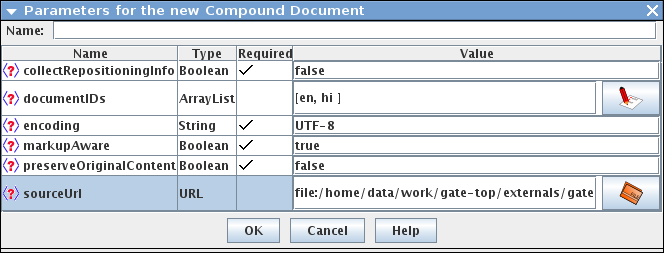
\includegraphics[width=\textwidth]{compound-document.png}
\caption{Compound Document}
\label{fig:compound-document}
\end{center}
\end{figure}

Compound document provides various methods that help in accessing their 
individual members.

\begin{small}\begin{verbatim}
public Document getDocument(String docid);
\end{verbatim}\end{small}

The following method returns a map of documents where the key is a document ID
and the value is its respective document.

\begin{small}\begin{verbatim}
public Map getDocuments();
\end{verbatim}\end{small}

Please note that only one member document in a compound document can have focus 
set on it.  Then all the standard document methods of gate.Document interface
apply to the document with focus set on it. For example, if there are two 
documents, `hi' and `en', and the focus is set on the document `hi' then the
getAnnotations() method will return a default annotation set of the
`hi' document.  One can use the following method to switch the focus
of a compound document to a different document:

\begin{small}\begin{verbatim}
public void setCurrentDocument(String documentID);
public Document getCurrentDocument();
\end{verbatim}\end{small}

As explained above, new documents can be added to or removed from the
compound document using the following method:

\begin{small}\begin{verbatim}
public void addDocument(String documentID, Document document);
public void removeDocument(String documentID);
\end{verbatim}\end{small}

The following code snippet demonstrates how to create a new compound document
using GATE Embedded:

\begin{lstlisting}

// step 1: initialize GATE 
Gate.init(); 
 
// step 2: load the Alignment plugin 
File alignmentHome = new File(Gate.getPluginsHome(),"Alignment"); 
Gate.getCreoleRegister().addDirectory(alignmentHome.toURL()); 
 
// step 3: set the parameters 
FeatureMap fm = Factory.newFeatureMap(); 
 
// for example you want to create a compound document for 
// File.id1.xml and File.id2.xml 
List docIDs = new ArrayList(); 
docIDs.add("id1"); 
docIDs.add("id2"); 
fm.put("documentIDs", docIDs); 
fm.put("sourceUrl", new URL("file:///url/to/File.id1.xml")); 
 
// step 4: finally create an instance of compound document 
Document aDocument = (gate.compound.CompoundDocument) 
    Factory.createResource("gate.compound.impl.CompoundDocumentImpl", fm);  
\end{lstlisting}

%%%%%%%%%%%%%%%%%%%%%%%%%%%%%%%%%%%%%%%%%%%%%%%%%%%%%%%%%%%%%%%%%%%%%%%%%%%%%
\subsect[sec:alignment:compoundDocFromXml]{CompoundDocumentFromXml}
%%%%%%%%%%%%%%%%%%%%%%%%%%%%%%%%%%%%%%%%%%%%%%%%%%%%%%%%%%%%%%%%%%%%%%%%%%%%%

As described later in the chapter, the entire compound document can be saved
in a single xml file.  In order to load such a compound document from the saved
xml file, we provide a language resource called CompoundDocumentFromXml.  This
is same as the Compound Document.  The only difference is in the parameters 
needed to instantiate this resource.  This LR requires only one parameter called
{\tt compoundDocumentUrl}.  The parameter is the url to the xml file.

%%%%%%%%%%%%%%%%%%%%%%%%%%%%%%%%%%%%%%%%%%%%%%%%%%%%%%%%%%%%%%%%%%%%%%%%%%%%%
\subsect[sec:alignment:compunddoceditor]{Compound Document Editor}
%%%%%%%%%%%%%%%%%%%%%%%%%%%%%%%%%%%%%%%%%%%%%%%%%%%%%%%%%%%%%%%%%%%%%%%%%%%%%

The compound document editor is a visual resource (VR) associated with
the compound document. The VR contains several tabs - each
representing a different member of the compound document.  All
standard functionalities such as GATE document editor, with all its
add-on plugins such as AnnotationSetView, AnnotationsList,
coreference editor etc., are available to be used with each individual
member.

Figure \ref{fig:compound-document-editor} shows a compound document
editor with English and Hindi documents as members of the compound
document.

\begin{figure}[ht]
\begin{center}
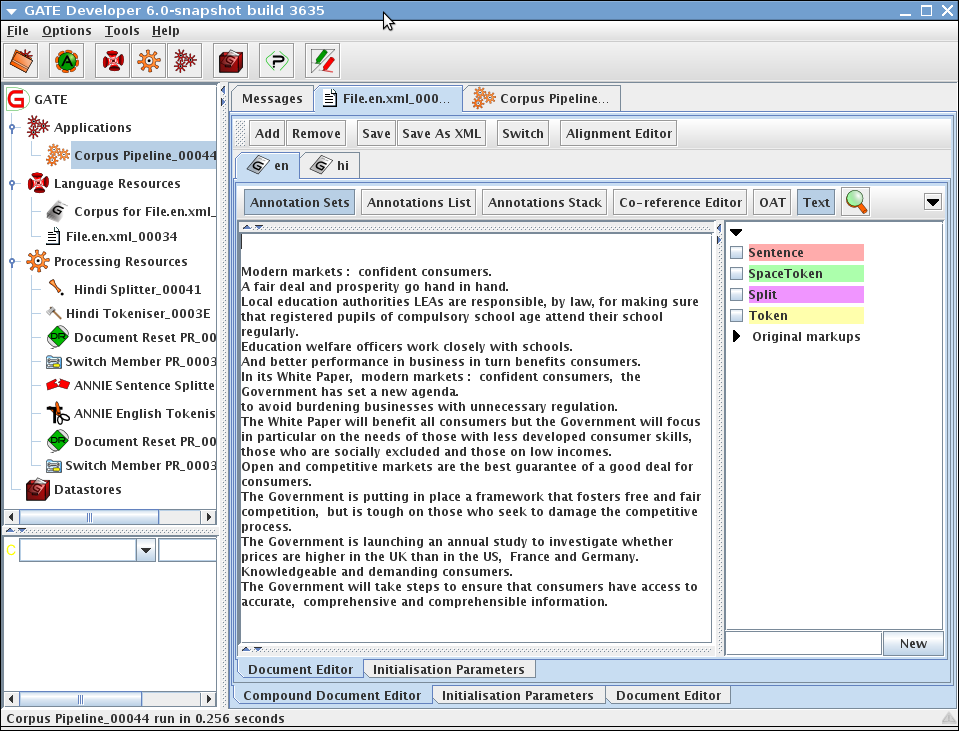
\includegraphics[width=\textwidth]{compound-document-editor.png}
\caption{Compound Document Editor}
\label{fig:compound-document-editor}
\end{center}
\end{figure}

As shown in the figure \ref{fig:compound-document-editor}, there are several
buttons at the top of the editor that provide different functionalities.  For
instance, the {\tt Add} button, allows adding a new member document to the
compound document. The {\tt Remove} button removes the current visible member 
from the document.  The buttons {\tt Save} and {\tt Save As XML} allow saving 
the documents individually and in a single xml document respectively.  The
{\tt Switch} button allows changing focus of the compound document from one
member to the other (this functionality is explained later). Finally, the {\tt
Alignment Editor} allows one to start the alignment editor to align text.

%%%%%%%%%%%%%%%%%%%%%%%%%%%%%%%%%%%%%%%%%%%%%%%%%%%%%%%%%%%%%%%%%%%%%%%%%%%%%
\subsect[sec:alignment:compositedoc]{Composite Document}
%%%%%%%%%%%%%%%%%%%%%%%%%%%%%%%%%%%%%%%%%%%%%%%%%%%%%%%%%%%%%%%%%%%%%%%%%%%%%

The composite document allows users to merge the texts of member documents and 
keep the merged text linked with their respective member documents.  In other 
words, if users make any change to the composite document (e.g. add new 
annotations or remove any existing annotations), the relevant effect is made to 
their respective documents.

A PR called CombineMembersPR allows creation of a new composite
document.  It asks for a class name that implements the
CombiningMethod interface.  The CombiningMethod tells the
CombineMembersPR how to combine texts and create a new composite
document.

For example, a default implementation of the CombiningMethod, called
DefaultCombiningMethod, takes the following parameters and puts the
text of the compound document's members into a new composite document.

\begin{small}\begin{verbatim}
unitAnnotationType=Sentence
inputASName=Key
copyUnderlyingAnnotations=true;
\end{verbatim}\end{small}

The first parameter tells the combining method that it is the `Sentence'
annotation type whose text needs to be merged and it should be taken from the
`Key' annotation set (second parameter) and finally all the underlying
annotations of every Sentence annotation must be copied in the composite
document.

If there are two members of a compound document (e.g. `hi' and
`en'), given the above parameters, the combining method finds out
all the annotations of type Sentence from each document and sorts them
in ascending order, and one annotation from each document is put one
after another in a composite document. This operation continues until
all the annotations have been traversed.

\begin{small}\begin{verbatim}
Document en     Document hi
Sen1            Shi1
Sen2            Shi2
Sen3            Shi3

Document Composite
Sen1
Shi1
Sen2
Shi2
Sen3
Shi3
\end{verbatim}\end{small}

The composite document also maintains a mapping of text offsets such
that if someone adds a new annotation to or removes any annotation
from the composite document, they are added to or removed from their
respective documents. Finally the newly created composite document
becomes a member of the same compound document.

%%%%%%%%%%%%%%%%%%%%%%%%%%%%%%%%%%%%%%%%%%%%%%%%%%%%%%%%%%%%%%%%%%%%%%%%%%%%%
\subsect[sec:alignment:deletemembers]{DeleteMembersPR}
%%%%%%%%%%%%%%%%%%%%%%%%%%%%%%%%%%%%%%%%%%%%%%%%%%%%%%%%%%%%%%%%%%%%%%%%%%%%%

This PR allows deletion of a specific member of the compound document.
It takes a parameter called `documentID' and deletes a document with
this name.

%%%%%%%%%%%%%%%%%%%%%%%%%%%%%%%%%%%%%%%%%%%%%%%%%%%%%%%%%%%%%%%%%%%%%%%%%%%%%
\subsect[sec::alignment:switchmembers]{SwitchMembersPR}
%%%%%%%%%%%%%%%%%%%%%%%%%%%%%%%%%%%%%%%%%%%%%%%%%%%%%%%%%%%%%%%%%%%%%%%%%%%%%

As described above, only one member of the compound document can have
focus set on it. PRs trying to use the getDocument() method get a pointer to the
compound document; however all the other methods of the compound
document give access to the information of the document member with
the focus set on it. So if user wants to process a particular member of the
compound document with some PRs, s/he should use the SwitchMembersPR
that takes one parameter called documentID and sets focus to the
document with that specific id.

%%%%%%%%%%%%%%%%%%%%%%%%%%%%%%%%%%%%%%%%%%%%%%%%%%%%%%%%%%%%%%%%%%%%%%%%%%%%%
\subsect[sec:alignment:saveasxml]{Saving as XML}
%%%%%%%%%%%%%%%%%%%%%%%%%%%%%%%%%%%%%%%%%%%%%%%%%%%%%%%%%%%%%%%%%%%%%%%%%%%%%

Calling the toXml() method on a compound document returns the XML
representation of the member which has focus.  However, GATE Developer
provides an option to save all member documents in different files.
This option appears in the options menu when the user right-clicks on
the compound document. The user is asked to provide a name for the
directory in which all the members of the compound document will be
saved in separate files.

It is also possible to save all members of the compound document in a
single XML file. The option, `Save in a single XML Document', also
appears in the options menu. After saving it in a single XML document,
the user can use the option `Compound Document from XML' to load the
document back into GATE Developer.

%%%%%%%%%%%%%%%%%%%%%%%%%%%%%%%%%%%%%%%%%%%%%%%%%%%%%%%%%%%%%%%%%%%%%%%%%%%%%
\subsect[sec:alignment:editor]{Alignment Editor}
%%%%%%%%%%%%%%%%%%%%%%%%%%%%%%%%%%%%%%%%%%%%%%%%%%%%%%%%%%%%%%%%%%%%%%%%%%%%%

Inspired by various tools, we have implemented a new version of alignment editor
that is comprised of several new features. We preserve standard ways of aligning
text but at the same time provide advanced features that can be used for 
facilitating incremental learning. The alignment editor can be used for 
performing alignment at any annotation level. When performing alignment at word 
or sentence level, the texts being aligned need to be pre-processed in order to 
identify tokens and sentences boundaries.

Information about the alignments carried over the text of a compound document is
stored as a document feature in the compound document itself. Since the document
features are stored in a map, every object stored as a document feature needs to
have a unique name that identifies that feature. There is no limit on how many 
features one can store provided they all have different names.  This allows 
storing alignment information, carried out at different levels, in separate 
alignment instances.  For example, if a user is carrying out alignment at a word
level, he/she can store it in an alignment object with a name 
{\tt word-alignment}.  Similarly, sentence alignment information can be stored 
with a name {\tt sentence-alignment}.  If multiple users are annotating the same
document, alignments produced by different users can be stored with different 
names (e.g. {\tt word-alignment-user1}, {\tt word-alignment-user2} etc.). {\tt 
Alignment} objects can be used for:

\begin{itemize}
\item aligning and unaligning two annotations;
\item checking if the two annotations are aligned with each other;
\item obtaining all the aligned annotations in a document;
\item obtaining all the annotations that are aligned to a particular annotation.
\end{itemize}

Given a compound document containing a source and a target document, the 
alignment editor starts in the alignment viewer mode. In this mode the texts
of the two documents are shown side-by-side in parallel windows. The purpose 
of the alignment viewer is to highlight the annotations that are already aligned.
The figure \ref{fig:alignment-viewer} shows the alignment viewer.  In this case
the selected documents are English and Hindi, titled as {\tt en} and {\tt hi} 
respectively.

\begin{figure}[ht]
\begin{center}
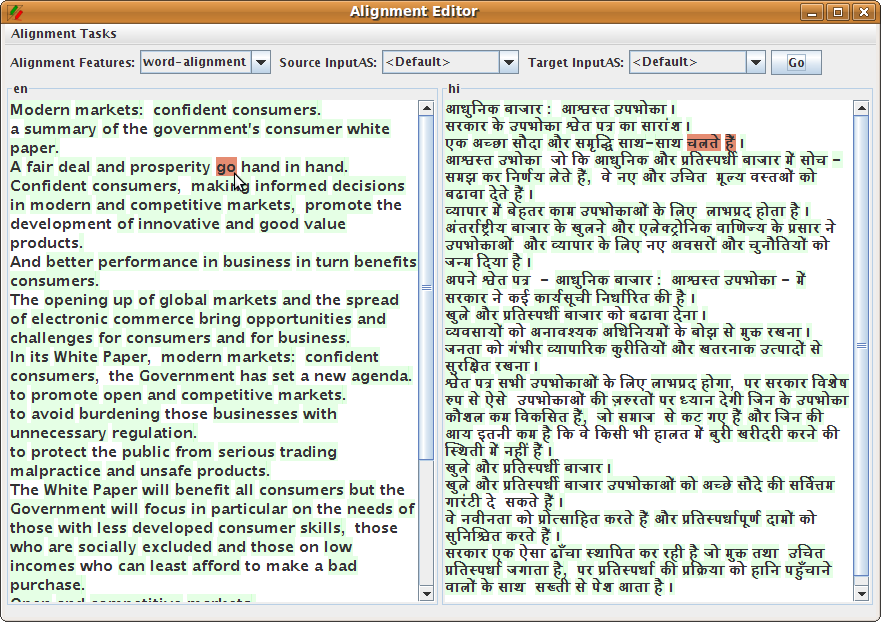
\includegraphics[width=\textwidth]{alignment-viewer.png}
\caption{Alignment Viewer}
\label{fig:alignment-viewer}
\end{center}
\end{figure}

To see alignments, user needs to select the alignment object that he/she wants 
to see alignments from.  Along with this, user also needs to select annotation 
sets - one for the source document and one for the target document. Given 
these parameters, the alignment viewer highlights the annotations that belong 
to the selected annotation sets and have been aligned in the selected alignment
object.   When the mouse is placed on one of the aligned annotations, the 
selected annotation and the annotations that are aligned to the selected 
annotation are highlighted in red. In this case (see figure 
\ref{fig:alignment-viewer}) the word {\tt go} is aligned with the words {\it 
chalate hein}. 

Before the alignment process can be started, the tool needs to know few 
parameters about the alignment task.

{\bf Unit Of Alignment:} this is the annotation type that users want to 
perform alignment at. {\bf Data Source:} generally, if performing a word 
alignment task, people consider a pair of aligned sentences one at a time and 
align words within sentences. If the sentences  are annotated, for example as 
{\tt Sentence}, the {\tt Sentence} annotation type is called {\bf Parent of 
Unit of Alignment}.  The {\tt Data Source} contains information about the 
aligned parents of unit of alignment. In this case, it would refer to the 
alignment object that contains alignment information about the annotations of 
type {\tt Sentence}. The editor iterates through the aligned sentences and forms
pairs of parent of unit of alignments to be shown to the user one by one.  If 
user does not provide any data source, a single pair is formed containing entire
documents. {\bf Alignment Feature Name:} this is the name given to the alignment 
object where the information about new alignments is stored.

The purpose of the alignment viewer is to highlight the annotations that are 
already aligned. The editor comes with three different views for performing 
alignment which the user can select at the time of creating a new alignment 
task: {\tt the Links view} (see \ref{fig:links-view} - suitable for character, 
word and phrase level alignments), {\tt the Parallel view} (see 
\ref{fig:parallel-view} - suitable for annotations which have longer texts, e.g.
sentences, paragraphs, sections)  and {\tt the Matrix view} (see 
\ref{fig:matrix-view}) - suitable for character, word and phrase level alignment. 

Let us assume that the user wants to align words in sentences using the {\tt 
Links view}.  The first thing he needs to do is to create a new Alignment task.
This can be achieved by clicking on the {\tt File} menu and selecting the {\tt
New Task} option.  User is asked to provide certain parameters as discussed 
above.  The editor also allows to store task configurations in an xml file which
can be at later stage reloaded in the alignment editor. Also, if there are more
than one task created, the editor allows users to switch between them.

To align one or more words in the source language with one or more words in the 
target language, the user needs to select individual words by clicking on them 
individually.  Clicking on words highlights them with an identical colour. Right
clicking on any of the selected words brings up a menu with the two default 
options: {\tt Reset Selection} and {\tt Align}. Different colours are used for 
highlighting different pairs of alignments. This helps distinguishing one set of
aligned words from other sets of aligned pairs. Also a link between the aligned 
words in the two texts is drawn to show the alignment. To unalign, user needs to
right click on the aligned words and click on the {\tt Remove Alignment} option. 
Only the word on which user right-clicks is taken out of the alignment and rest 
of the words in the pair remain unaffected.  We use the term {\tt Orphaned 
Annotation} to refer to the annotation which does not have any alignment in the 
target document.  If after removing an annotation from alignment pair, there are
any orphaned annotations in the alignment pair, they are unaligned too.

\begin{figure}[ht]
\begin{center}
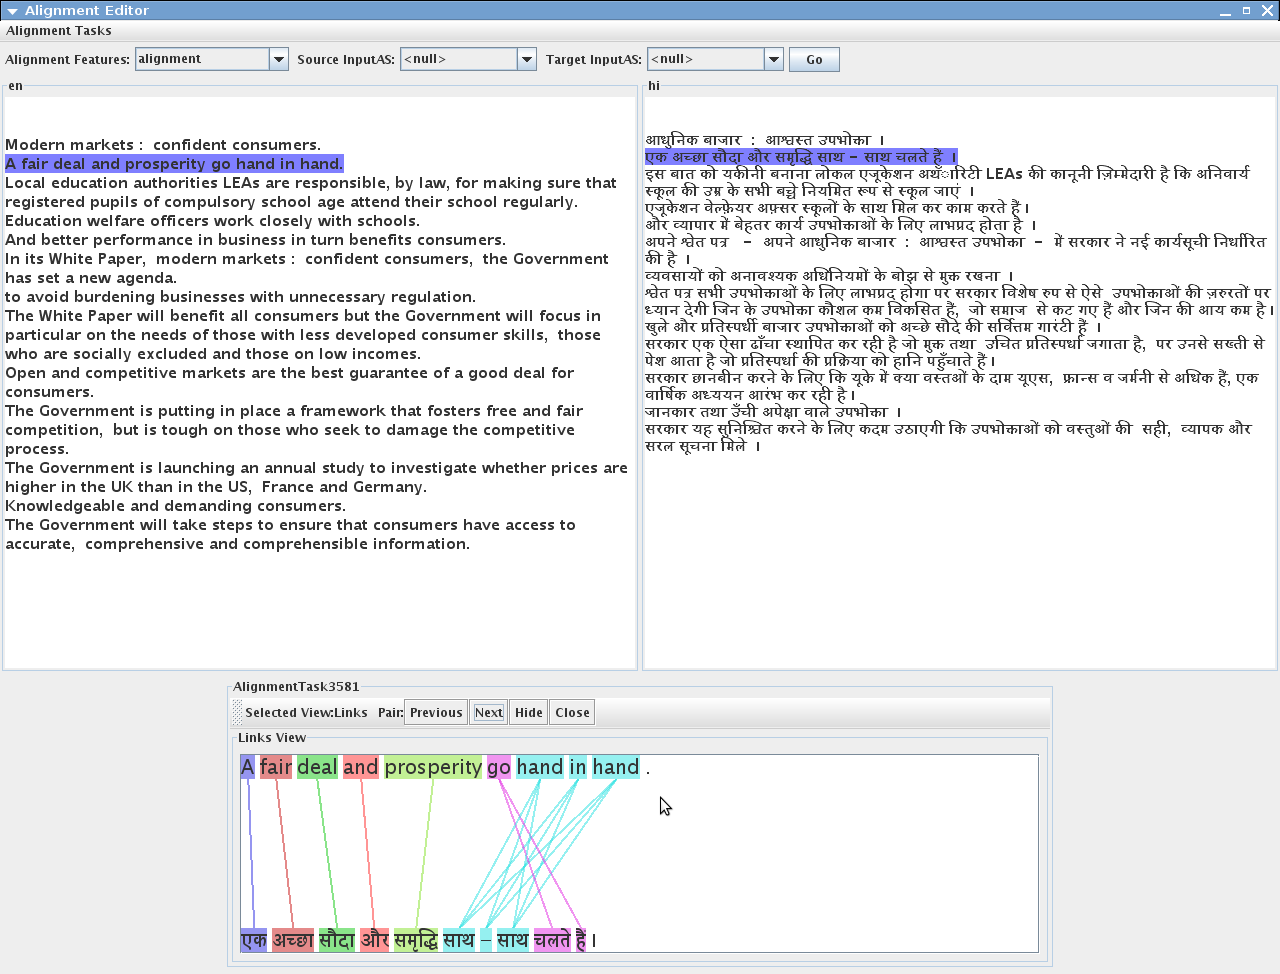
\includegraphics[width=\textwidth]{links-view.png}
\caption{Links View}
\label{fig:links-view}
\end{center}
\end{figure}

\begin{figure}[ht]
\begin{center}
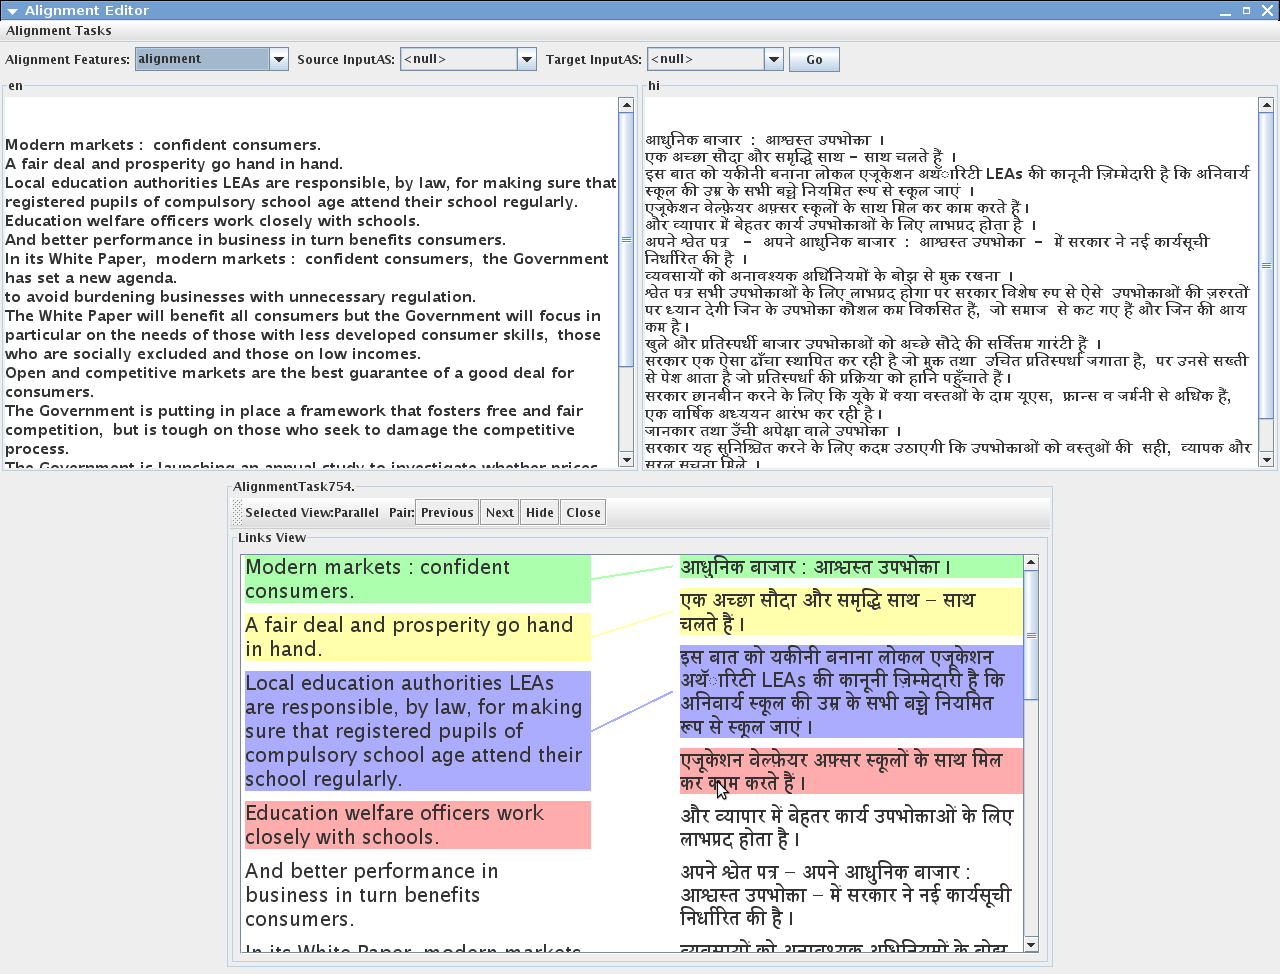
\includegraphics[width=\textwidth]{parallel-view.png}
\caption{Parallel View}
\label{fig:parallel-view}
\end{center}
\end{figure}

\begin{figure}[ht]
\begin{center}
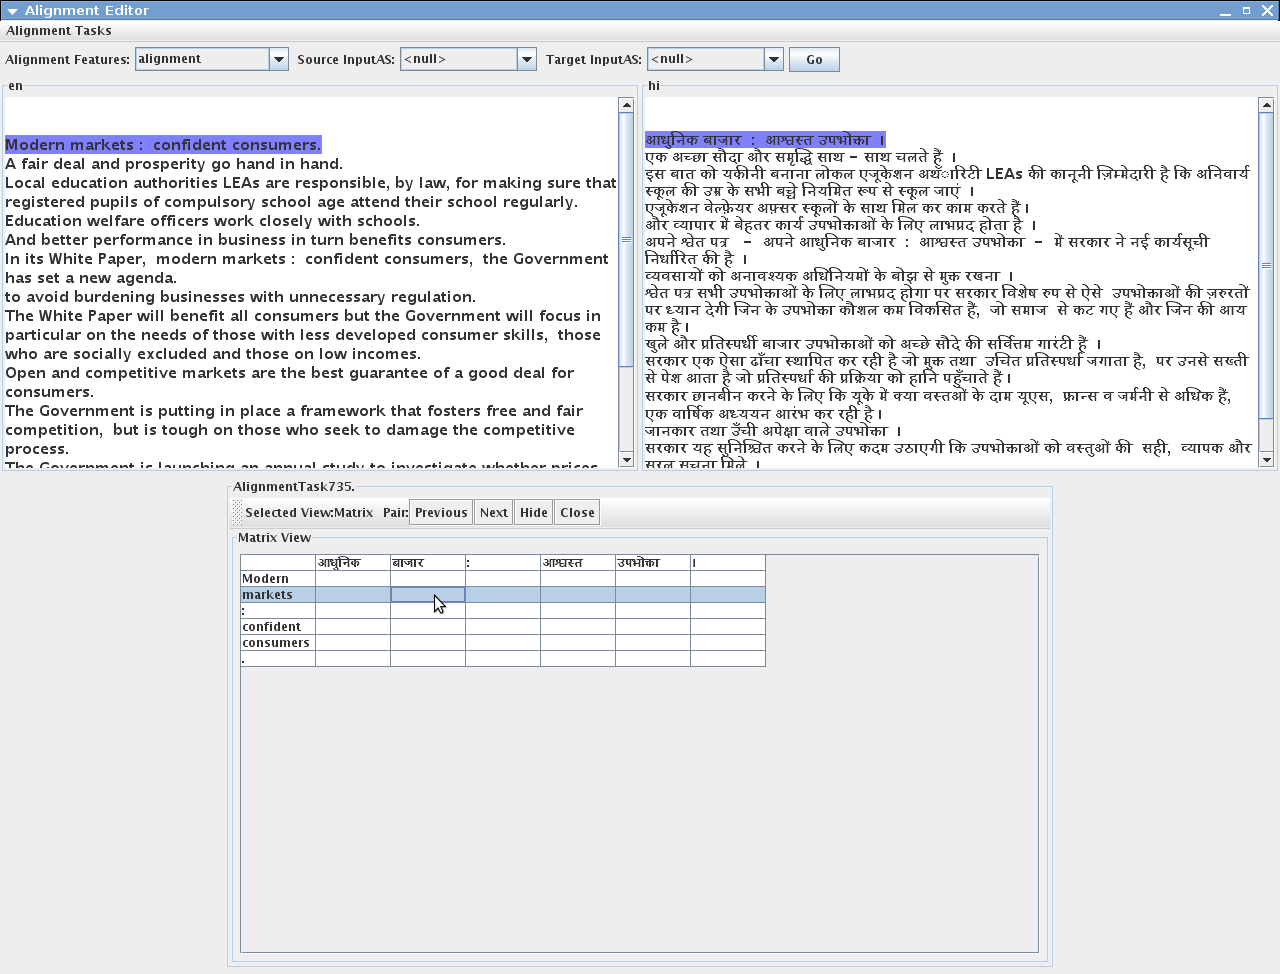
\includegraphics[width=\textwidth]{matrix-view.png}
\caption{Matrix View}
\label{fig:matrix-view}
\end{center}
\end{figure}


%%%%%%%%%%%%%%%%%%%%%%%%%%%%%%%%%%%%%%%%%%%%%%%%%%%%%%%%%%%%%%%%%%%%%%%%%%%%%
\subsubsect[sec:alignment:editor:advanced-features]{Advanced Features}
%%%%%%%%%%%%%%%%%%%%%%%%%%%%%%%%%%%%%%%%%%%%%%%%%%%%%%%%%%%%%%%%%%%%%%%%%%%%%

The options {\tt Align}, {\tt Reset Selection} and {\tt Remove Alignment} are 
available by default. The {\tt Align} and the {\tt Reset Selection} options 
appear when user wants to align new annotations.  The {\tt Remove Alignment} 
option only appears when user right clicks on the already aligned annotations.
The first two actions are available when there is at least one annotation 
selected in the source language and another one is selected in the target 
language.  Apart from these three basic actions, the editor also allows adding 
more actions to the editor.

There are four different types of actions: actions that should be taken before
the user starts aligning words ({\tt PreDisplayAction}); actions that should be 
taken when the user aligns annotations ({\tt AlignmentAction}); the actions
that should be taken when the user has completed aligning all the words in the 
given sentence pair ({\tt FinishedAlignmentAction}) and the actions to publish
any data or statistics to the user. For example, to help users in the alignment 
process by suggesting word alignments, one may want to wrap a pre-trained 
statistical word alignment model as PreDisplayAction. Similarly, actions of the
type AlignmentAction can be used for submitting examples to the model in order 
for the model to update itself. When all the words in a sentence pair are 
aligned, one may want to sign off the pair and take actions such as comparing 
all the alignments in that sentence pair with the alignments carried out by some
other user for the same pair. Similarly, while collecting data in the background,
one might want to display some information to the user (e.g. statistics for the
collected data or some suggestions that help users in the alignment process).

When users click on the {\tt next} or the {\tt previous} button, the editor 
obtains the next or the previous pair that needs to be shown from the data 
source.  Before the pair is displayed in the editor, the editor calls the 
registered instances of the {\tt PreDisplayAction} and the current pair object
is passed onto the instances of {\tt PreDisplayAction}. Please note that this
only happens when the pair is not already signed off. Once the instances of 
{\tt PreDisplayAction} have been executed, the editor collects the alignment
information from the compound document and displays it in the editor.

As explained earlier, when users right click on units of alignment in the editor
a popup menu with default options (e.g. Align, Reset Selection and Remove
Alignment) is shown.  The editor allows adding new actions to this menu.  It is 
also possible that users may want to take extra actions when they click on any 
of the {\tt Align} or the {\tt Remove Alignment} options.  The {\tt 
AlignmentAction} makes it possible to achieve this.  Below we list some of the 
parameters of the AlignmenAction. The implementation is called depending on 
these parameters.

\begin{itemize}
\item {\tt invokeForAlignedAnnotation} - the action appears in the options menu
when user right clicks on the aligned annotation.
\item {\tt invokeForHighlightedUnalignedAnnotation} - the action appears in the
options menu when user right clicks on a highlighted but unaligned annotation.
\item {\tt invokeForUnhighlightedUnalignedAnnotation} - the action appears in
the options menu when user right clicks on an unhighlighted and unaligned 
annotation.
\item {\tt invokeWithAlignAction} - the action is executed whenever user aligns
some annotations.
\item {\tt invokeWithRemoveAction} - the action is executed whenever user removes
any alignment.
\item {\tt caption} - in case of the first three options, the caption is used in
the options menu.  In case of the fourth and the fifth options, the caption 
appears as a check box under the {\tt actions tab}.
\end{itemize}

These methods can be used for, for example, building up a dictionary in the 
background while aligning word pairs.  Before users click on the next button, 
they are asked if the pair they were aligning has been aligned completely (i.e. 
signed off for further alignment). If user replies yes to it, the actions 
registered as FinishedAlignmentAction are executed one after the other. This 
could be helpful, for instance, to write an alignment exporter that exports 
alignment results in an appropriate format or to update the dictionary with
new alignments. 

Users can point the editor to a file that contains a list of actions and 
parameters needed to initialize them.  A configuration file is a simple text file
with fully-qualified class name, and required parameters specified in it.
Below we give an example of such a configuration file.

\begin{small}\begin{verbatim}
gate.alignment.actions.AlignmentCache,$relpath$/align-cache.txt,root
\end{verbatim}\end{small}

The first argument is the name of the class that implements one of the actions
described above.  The second parameter is the name of the file in which the
alignment cache should store its results. Finally, the third argument instructs
the alignment cache to store root forms of the words in the dictionary so that
different forms of the same words can be matched easily.  All the parameters 
(comma separated) after the class name are passed to the action. The {\tt relpath}
parameter is resolved at runtime.


{\tt AlignmentCache} is one such example of FinishedAlignmentAction and the
PreDisplayAction.  This is an inbuilt alignment cache in the editor which 
collects alignment pairs that the users annotate. The idea here is to cache such
pairs and later, align them automatically if they appear in subsequent pairs, 
thus reducing the efforts of humans to annotate the same pair again.  By default
the alignment cache is disabled. Users wishing to enable it should look into the
plugins/Alignment/resources/actions.conf and uncomment the appropriate line.

Users wishing to implement their own actions should refer to the implementation
of the AlignmentCache.

%%%%%%%%%%%%%%%%%%%%%%%%%%%%%%%%%%%%%%%%%%%%%%%%%%%%%%%%%%%%%%%%%%%%%%%%%%%%%
\subsect[sec:alignment:exportFilesAndAlignments]{Saving Files and Alignments}
%%%%%%%%%%%%%%%%%%%%%%%%%%%%%%%%%%%%%%%%%%%%%%%%%%%%%%%%%%%%%%%%%%%%%%%%%%%%%

A compound document can have more than one member documents, the alignment 
information stored as a document feature and more than one alignment features.
The framework allows users to store the whole compound document in a single XML 
file.  The XML file contains all the necessary information about the compound
document to load it back in Gate and bring it to the state the compound document
was when saving the document as XML.  It contains XML produced for each and 
every member document of the compound document and the details of the document 
features set on the compound document.  XML for each member document includes 
XML elements for its content; annotations sets and annotations; document 
features set on individual member document and the id given to this document as 
as member of the compound document.  Having a single XML file makes it possible
to port the entire file from one destination to the others easily.

Apart from this, the framework has an alignment exporter. Using the alignment 
exporter, it is possible to store the alignment information in a separate XML 
file. For example, once the annotators have aligned documents at a word level, 
the alignment information about both the unit and the parent of unit annotations 
can be exported to an XML file.  Figure \ref{fig:wa-xml-output} shows an XML 
file with word alignment information in it.

\begin{figure}[ht]
\centering
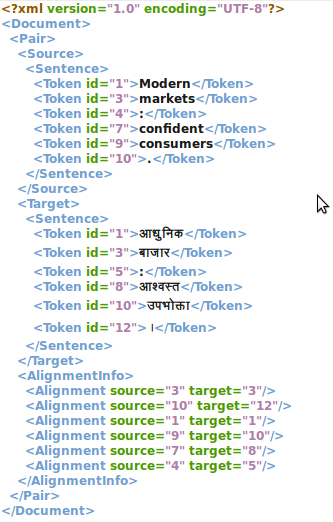
\includegraphics[width=5cm]{wa-xml-output.png}
\caption{Word Alignment XML File} 
\label{fig:wa-xml-output}
\end{figure}

When aligning words in sentences, it is possible to have one or more source 
sentences aligned with one or more target sentences in a pair. This is achieved
by having {\tt Source} and {\tt Target} elements within the {\tt Pair} element
which can have one or more {\tt Sentence} elements in each of them. Each 
word or token within these sentences is marked with {\tt Token} element. 
Every {\tt Token} element has a unique id assigned to it which is used when 
aligning words.  It is possible to have 1:1 or 1:many and many:1 alignments.  
The {\tt Alignment} element is used for mentioning every alignment pair with 
{\tt source} and {\tt target} attributes that refer to one of the source token 
ids and one of the target document ids respectively.  For example, according to 
the first alignment entry, the source token  {\tt markets} with id 3 is aligned 
with the target token {\it bAzAr} with id 3. The exporter does not export any 
entry for the unaligned words.

%%%%%%%%%%%%%%%%%%%%%%%%%%%%%%%%%%%%%%%%%%%%%%%%%%%%%%%%%%%%%%%%%%%%%%%%%%%%%
\subsect[sec:alignment:segment-processing]{Section-by-Section Processing}
%%%%%%%%%%%%%%%%%%%%%%%%%%%%%%%%%%%%%%%%%%%%%%%%%%%%%%%%%%%%%%%%%%%%%%%%%%%%%

In this section, we describe a component that allows processing documents 
section-by-section. Processing documents this way is useful for many reasons:

For example, a patent document has several different sections but user is  
interested in processing only the `claims' section or the `technical details 
section'.  This is also useful for processing a large document where processing 
it as a single document is not possible and the only alternative is to divide 
it in several small documents to process them independently.  However, doing so 
would need another process that merges all the small documents and their 
annotations back into the original document. On the other hand, a webpage may 
contain profiles of different people. If the document has more than one person
with similar names, running the `Orthomatcher PR' on such a document would 
produce incorrect coreference chains.

All such problems can be solved by using a PR called `Segment Processing PR'.
This PR is distributed as part of the `Alignment' plugin.  User needs to 
provide the following four parameters to run this PR.

\begin{enumerate}
\item {\tt document:} This is the document to be processed.
\item {\tt analyser:} This can be a PR or a corpus controller that needs to be used for
processing the segments of the document.
\item {\tt segmentAnnotationType:} Sections of the documents (that need to be
processed) should be annotated with some annotation type and the type of such
annotation should be provided as the value to this parameter.
\item {\tt segmentAnnotationFeatureName} and {\tt segmentAnnotationFeatureValue:} 
If user has provided values for these parameters, only the annotations with the 
sepcified feature name and feature value are processed with the Segment Processing PR.
\item {\tt inputASName:} This is the name of the annotation set that contains
the segment annotations.
\end{enumerate}

Given these parameters, each span in the document that is annotated as the type
specified by the {\tt segmentAnnotationType} is processed independently.  

Given a corpus of publications, if you just want to process the abstract section
with the ANNIE application, please follow the following steps. It is assumed
that the boundaries of abstracts in all these publications are already 
identified. If not, you would have to do some processing to identify them prior 
to using the following steps. In the following example, we assume that the 
abstract boundaries have been annotated as `Abstract' annotations and stored 
under the `Original markups' annotation set.

Steps:
\begin{enumerate}
\item Create a new corpus and populate it with a set of publications that you 
would like to process with ANNIE.
\item Load the ANNIE application.
\item Load the `Alignment' plugin.
\item Create an instance of the `Segment Processing PR' by selecting it from
the list of processing resources.
\item Create a corpus pipeline.
\item Add the `Segment Processing PR' into the pipeline and provide the 
following parameters:
\begin{enumerate}
\item Provide the corpus with publication documents in it as a parameter to
the corpus controller.
\item Select the `ANNIE' controller for the `controller' parameter.
\item Type `Abstract' in the `segmentAnnotationType' parameter.
\item Type `Original markups' in the `inputASName' parameter.
\end{enumerate}
\item Run the application.
\end{enumerate}

Now, you should see that the ANNIE application has only processed the text in 
each document that was annotated as `Abstract'.
